\documentclass[a4paper,11pt]{article}

\usepackage[utf8]{inputenc}

\usepackage{graphicx}
\usepackage{caption}
\usepackage{subcaption}

\usepackage{pgfplots}
\pgfplotsset{compat=1.18} 

\usepackage{comment}

\usepackage{gensymb}

\begin{document}

\title{
  \textbf{Carbon} \\
  the source of atmospheric carbon dioxide levels
}
\author{Johan Montelius}
\date{\today}

\maketitle

\section*{Introduction}

The concentration of carbon dioxide levels have increased during the
last century and we have very good data that shows us the
concentration on a monthly basis during the last sixty years. The
reason is, given the current narrative, that this is all due to our
burning of fossil fuel. This article will present some data that, at
least will make it plausible that, this is not the whole story. In fact
it might be that we are only responsible to a lesser degree - if this
is correct then it might have consequences. 

\section*{Mauna Loa}

We start by examining the measurements of carbon dioxide
concentrations in the atmosphere from the Mauna Loa observatory on the
island of Hawaii. The data that we will use is the mean monthly
measurements from $1958$ to $2026$ (full years from $1959$ to
$2025$). If we plot these data we will see the classical {\em Keeling
  curve} as shown Fig.\ref{fig:maunaloa}-a. If we look at the changes
during a year we see "the earth breathing" - during the northern
hemisphere summer, the growth in vegetation decrease the amount of
carbon dioxide in the atmosphere which is later released during
winter.

\begin{figure}[t]
  \centering
  \hspace*{-4cm}
  \begin{subfigure}{.5\paperwidth}
    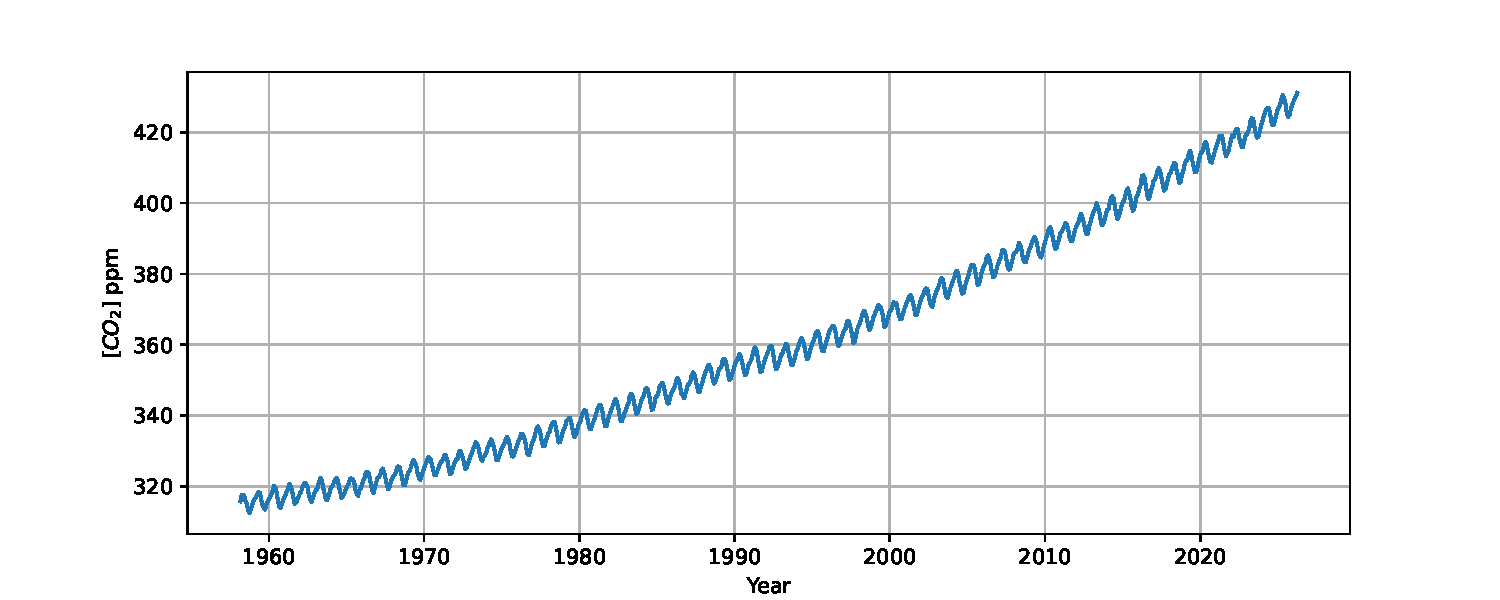
\includegraphics[scale=0.4]{../img/keeling.pdf}
    \caption{the Keeling curve}
  \end{subfigure}%
  \begin{subfigure}{.5\paperwidth}
    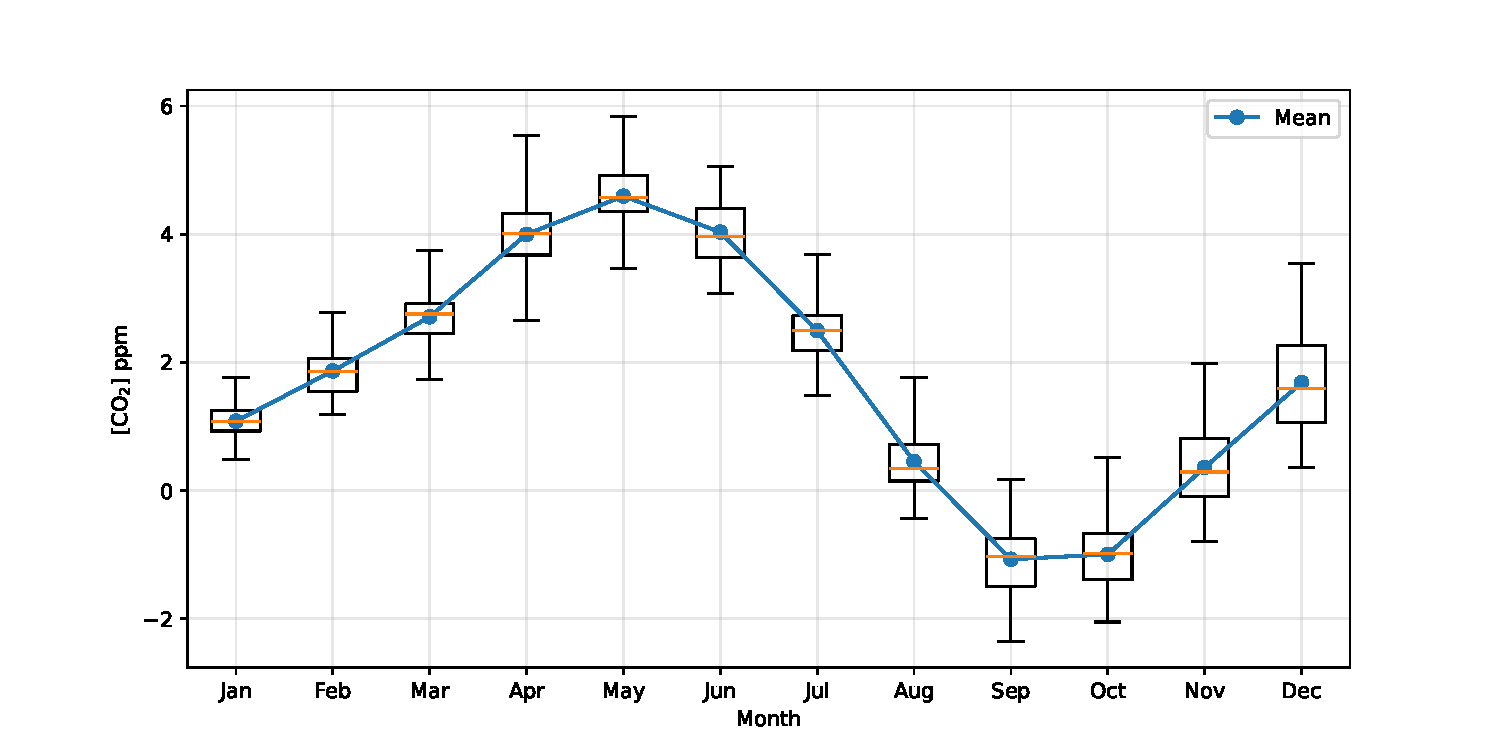
\includegraphics[scale=0.4]{../img/yearly-variations.pdf}
    \caption{variation during a year.}
  \end{subfigure}
  \caption{Carbon dioxide concentration in the atmosphere..}
  \label{fig:maunaloa}
\end{figure}

One interesting fact to note is that the yearly natural changes has a
range of more than five ppm. We will look at the final increase over a
year that is around 2 ppm. The changes during a year is thus larger
than the increase that we will investigate further.

\section*{Emissions}

We of course need data on the worlds yearly fossil fuel consumption
and this is of course nothing that can be measured. However, since
fossil fuels (coal, oil, gas) are globally traded there are reliable
data on production and consumption, and for our use these will be
sufficient.

I've chosen the data obtained from "Global Carbon Budget" which is a
provided by the University of Exeter. This compilation consists of
estimates of yearly fossil fuel consumption, divided by source, from
1850 up to 2024 (the data for 2025 is not yet provided). There are
other compilations but they do not vary much and for our purposes I
think the data is accurate enough.

If we look at Fig.\ref{fig:gcb}-a we see the yearly emissions in
giga-ton coal. We can note that emission up until 1950 were quite
modest compared to our emissions today. If we look at
Fig.\ref{fig:gcb}-b we see that the total accumulated emissions
between 1850 and 1958 is approximately 80 GtC which could be compared
to the emissions of 2024 alone that was in total 10 GtC i.e. today we
emit in one decade more than we have emitted between 1850 and 1958. 


\begin{figure}[ht!]
  \centering
  \hspace*{-4cm}
  \begin{subfigure}{.5\paperwidth}
    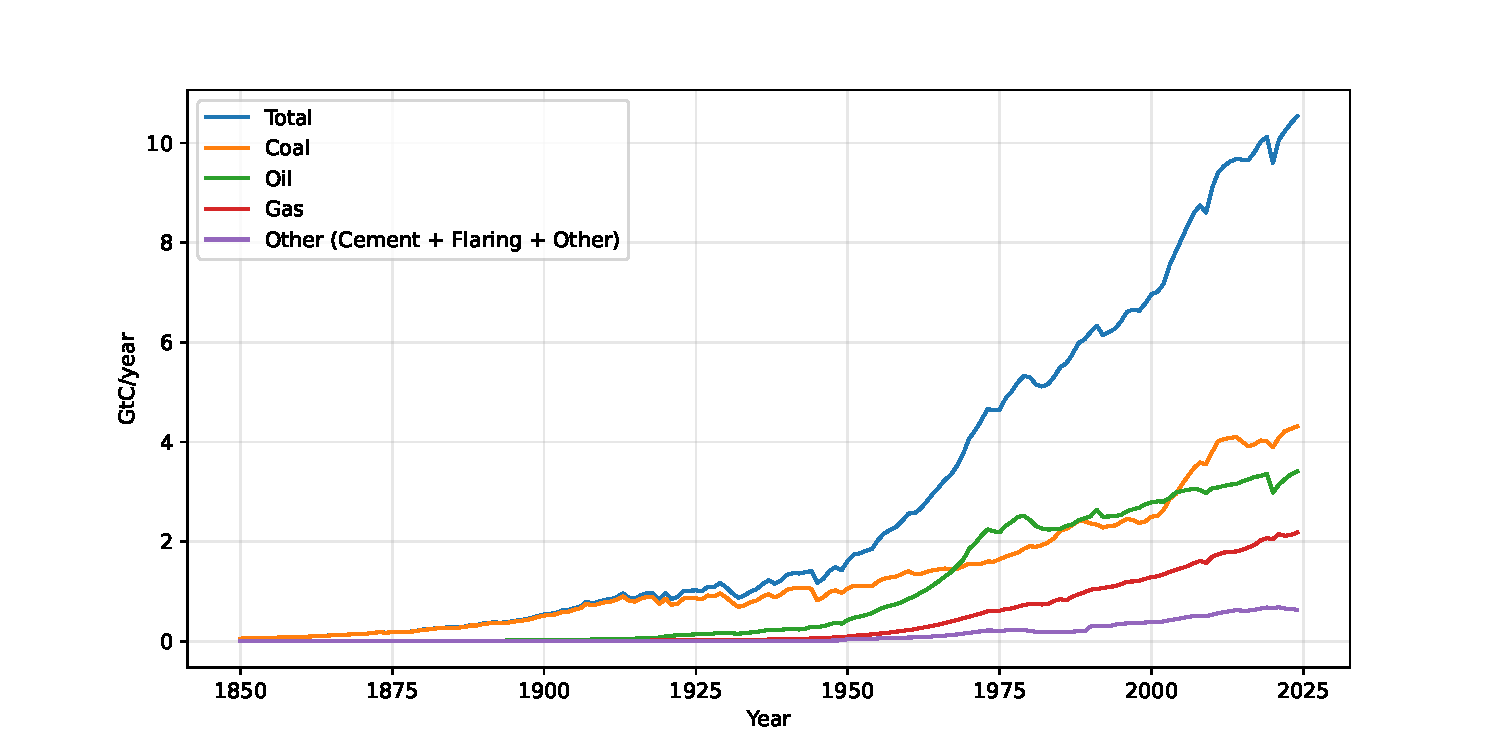
\includegraphics[scale=0.4]{../img/gcb.pdf}
    \caption{Yearly emissions}
  \end{subfigure}%
  \begin{subfigure}{.5\paperwidth}
    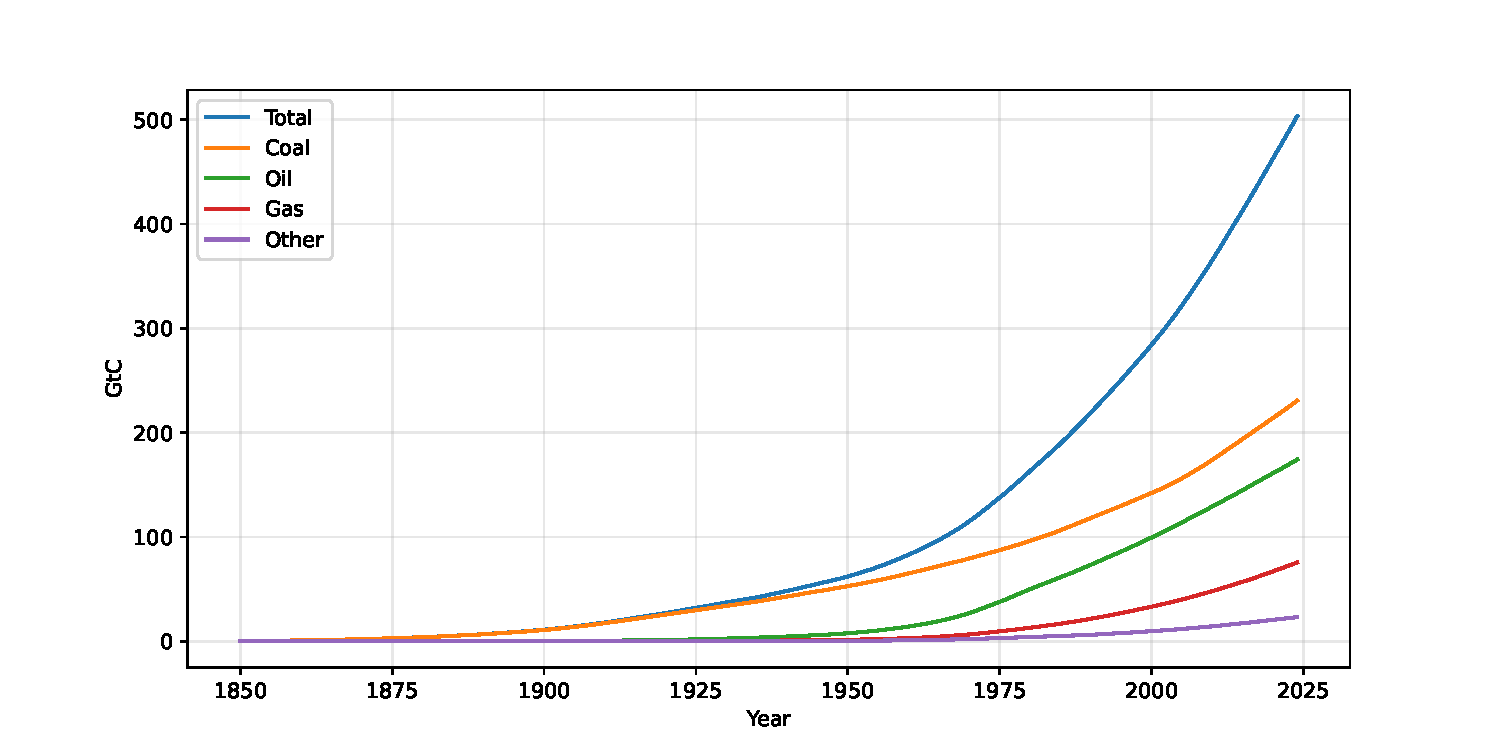
\includegraphics[scale=0.4]{../img/gcb-cum.pdf}
    \caption{Accumulated emissions}
  \end{subfigure}
  \caption{Global Carbon Budget: world fossil emissions.}
  \label{fig:gcb}
\end{figure}


\section*{Correlation}

One question we might ask is how well our emissions correlate with the
increase on carbon dioxide concentrations. We can convert our
emissions, that are measured on giga-ton of coal into concentration in
the atmosphere, in ppm, by dividing by $2.13$ (standard procedure use
by IPCC). The increase in concentration for a given year can of course
be calculated in various ways but why not use the December value minus
the previous December.

In Fig.\ref{fig:correlation} we see a scatter plot with linear
regression of the emissions and atmospheric increase. We can note that
the emissions in general are twice as high as the increase seen in the
atmosphere. The correlation is however not very strong, an $R^2$
value of $0.6$ is not very reassuring. An emission in one year of
approximately 3 ppm of carbon dioxide, corresponds to anything between
$0.5$ to almost $3$ ppm of increase. What is it that determines the
yearly increase; our emissions are - even though twice as high - not a
good predictor of the atmospheric increase.

\begin{figure}[ht!]
  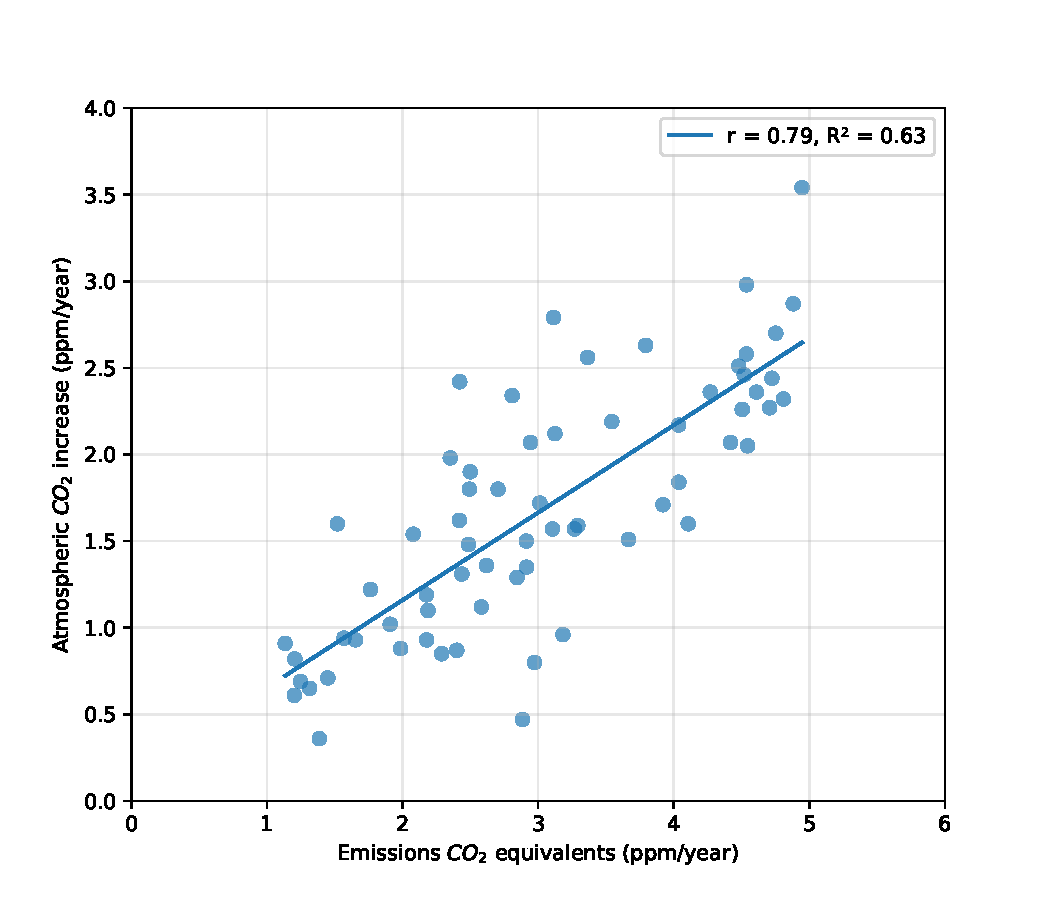
\includegraphics[scale=0.6]{../img/correlation.pdf}
  \caption{Correlation: emissions and atmospheric increase.}
  \label{fig:correlation}
\end{figure}

We could stop here and argue that there are a lot of things happening
but for sure - half of our emissions end up in the atmosphere. We could
also investigate things further; let's take a look at the temperature
over the same period.

\section*{Temperature}

When do not have any reliable numbers on the {\em global temperature}
but we do have several good estimates on how temperature has changed
over time. One source is "Global Land and Ocean Average Temperature
Departures" compiled and published by NOAA. The series extend back to
1850 but one must realize that the error bars are quite large when we
are talking about remote areas before the age of satellites. We could
have looked at the series published by University of Alabama in
Huntsville that are based sole on satellite data, but that series only
extends back to 1979.

If we look at Fig.\ref{fig:temperature} we see that the two series in
large agree. They have chosen different time periods as their base
but to a large extent they do agree (UAH has a wider variance). For
this discussion the difference does not matter that much and sin since we
have carbon dioxide levels from 1958 we choose the series from NOAA.

\begin{figure}[]
  \center
  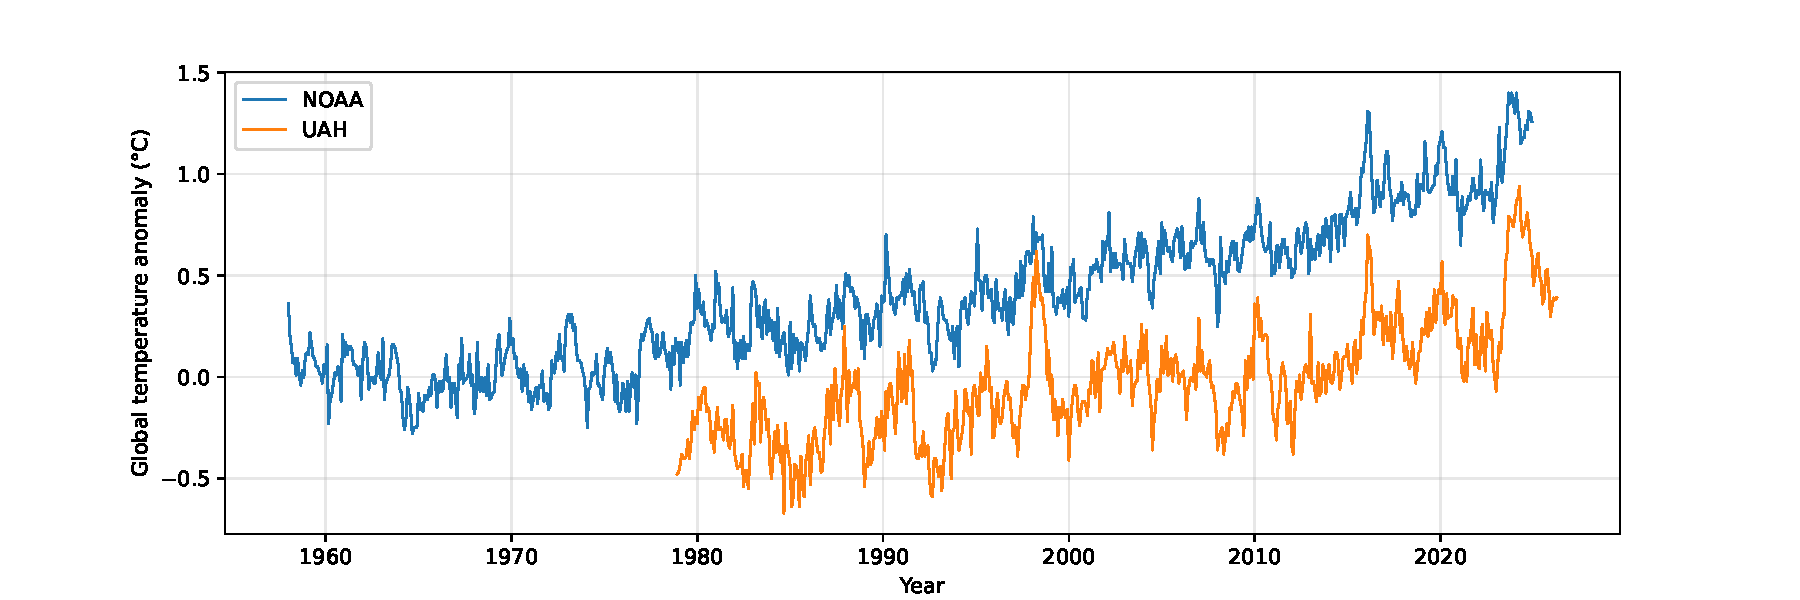
\includegraphics[scale=0.5]{../img/temperature.pdf}
  \caption{Global temperature anomalies}
  \label{fig:temperature}
\end{figure}

If we take the average of temperatures each year we can look at the
correlation with increase in carbon dioxide levels. The result is
shown in Fig.\ref{fig:temperature-ppm} and even though the correlation
is not very strong, $R^2$ is $0.72$ which is higher than what we had
for the correlation with fossil emissions. From a statistical point of
view, it would not be wrong to suspect that the temperature might
affect the carbon dioxide levels more than our emissions.

\begin{figure}[ht!]
  \center
  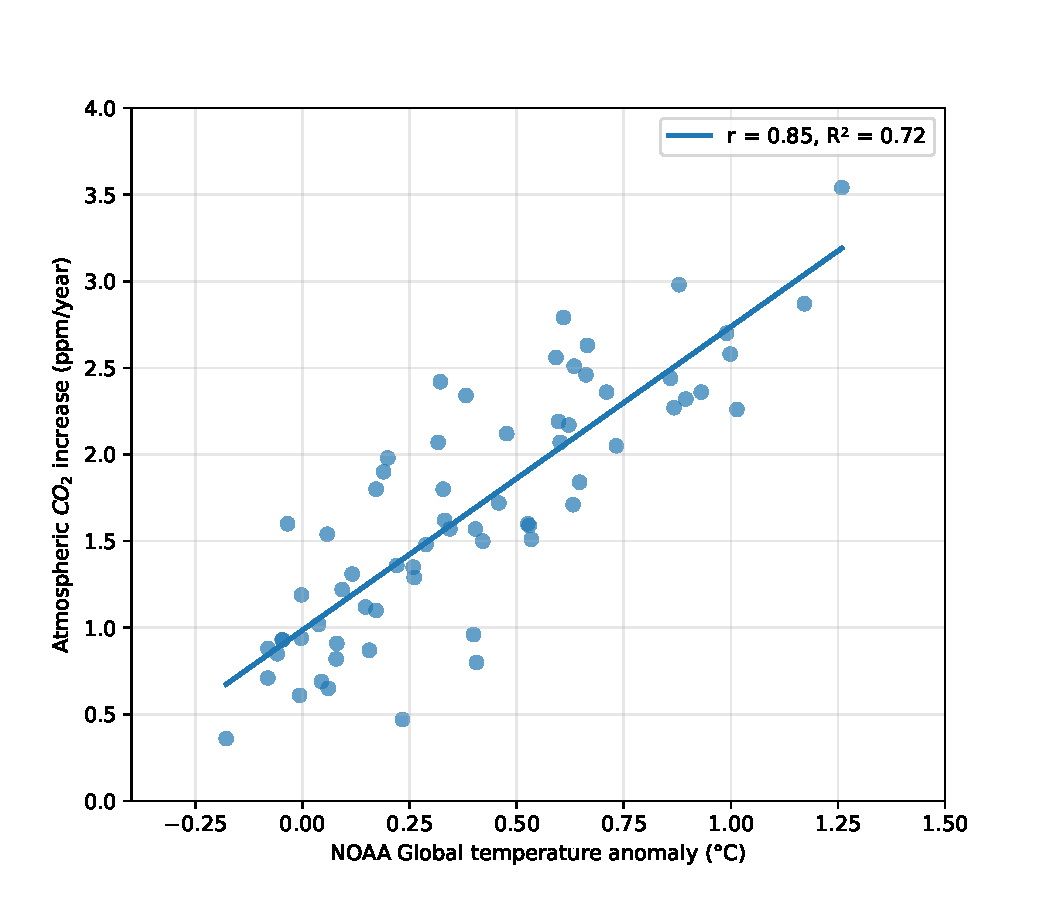
\includegraphics[scale=0.5]{../img/temperature-ppm.pdf}
  \caption{Correlation: temperature and atmospheric increase.}
  \label{fig:temperature-ppm}
\end{figure}

\section*{Regression}

Since we suspect that both emissions and temperature effect the carbon
dioxide levels we could of course do a regression analysis for:

$$ incr = k_t \times temp + k_e \times emi + const$$

The result is shown in Tab.\ref{tab:regression} and from this we would
conclude that the temperature is a far more important factor in
determining the increase in carbon dioxide levels. Given the regression
analysis it strangely enough seams that our emissions play no role at
all? 


\begin{table}[ht!]
\centering
\begin{tabular}{ c c c c c c  }
 \textbf{var} & \textbf{k} & \textbf{std err} & \textbf{t} & \textbf{P\textgreater[t]} & 95\% \\
\hline\\
const &         1.0013 &    0.238 &    4.198 &    0.000 &    [0.52, 1.48] \\
temp &          1.7765 &    0.407 &    4.369 &    0.000 &    [0.96, 2.59] \\
emi &          -0.0083 &    0.125 &   -0.066 &    0.947 &    [-0.26, 0.24] \\
\end{tabular}
\caption{Regression analysis.}
\label{tab:regression}
\end{table}

Before we draw any conclusions of this regression analysis we should
note that the temperature and yearly emissions are highly correlated
($0.947$). They both show an increase during the period and it might
be hard to separate the two. We also have a large constant factor that
hides the contribution from either the temperature or emissions or
both. The constant factor would however disappear if we used
temperature anomalies from the mid eighteen-hundreds when the global
average was half a degree lower.

The statistical model we now have:

$$ incr = 1.8 \times temp + 1$$

gives us that the carbon dioxide levels would stabilize if the
temperature dropped to a half degree below the NOAA reference period
(1901-2000). Is it possible that emissions play an insignificant role?


\section*{Model}

When first presented with the given model a normal reaction is that
"yes - temperature effect the yearly increase but the long term
increase is due to emissions". This might be true but the statistical
model we now have does correlate well with the yearly increases as shown in 
Fig.\ref{fig:recon}-a. If we integrate the statistical model and start from $315$ ppm we 
can explain the whole increase of atmospheric carbon dioxide over the period as seen in Fig.\ref{fig:recon}-b.

\begin{figure}[ht!]
  \centering
  \hspace*{-3cm}
  \begin{subfigure}{.5\paperwidth}
    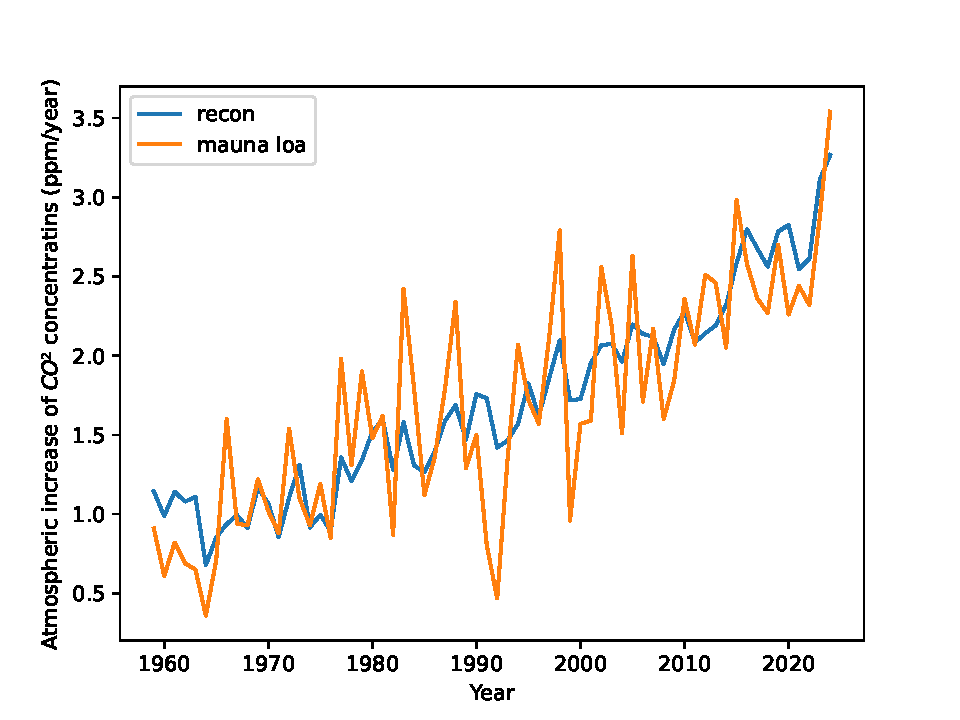
\includegraphics[scale=0.5]{../img/recon1.pdf}
    \caption{increase}
  \end{subfigure}%
  \begin{subfigure}{.5\paperwidth}
    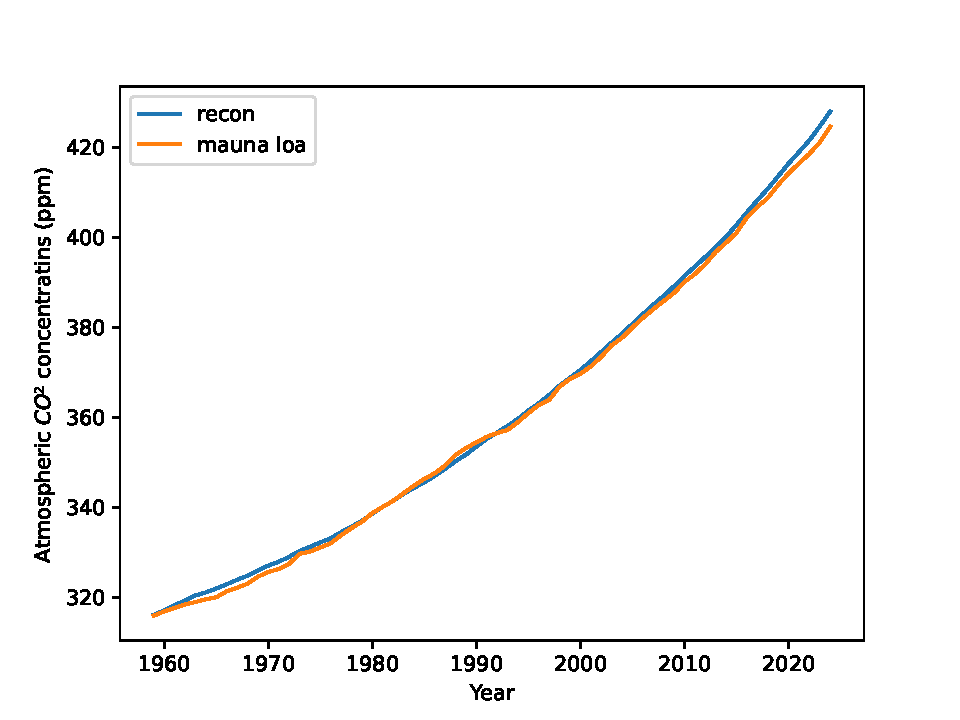
\includegraphics[scale=0.5]{../img/recon2.pdf}
    \caption{accumulated}
  \end{subfigure}
  \caption{Reconstruction of carbon dioxide levels}
  \label{fig:recon}
\end{figure}

The statistical model that we have now is of course not a physical
model of what is happening. It happens to be a good approximation of
the last sixty years but fails when we for example try to explain the
growth from $1850$ when carbon dioxide levels are believed to be
around $285$ ppm. The model will over shoot and land on a calculated
value of $470$ ppm where the current level is approximately $420$ ppm
as shown in Fig.\ref{fig:shoot}.


\begin{figure}[ht!]
  \center
  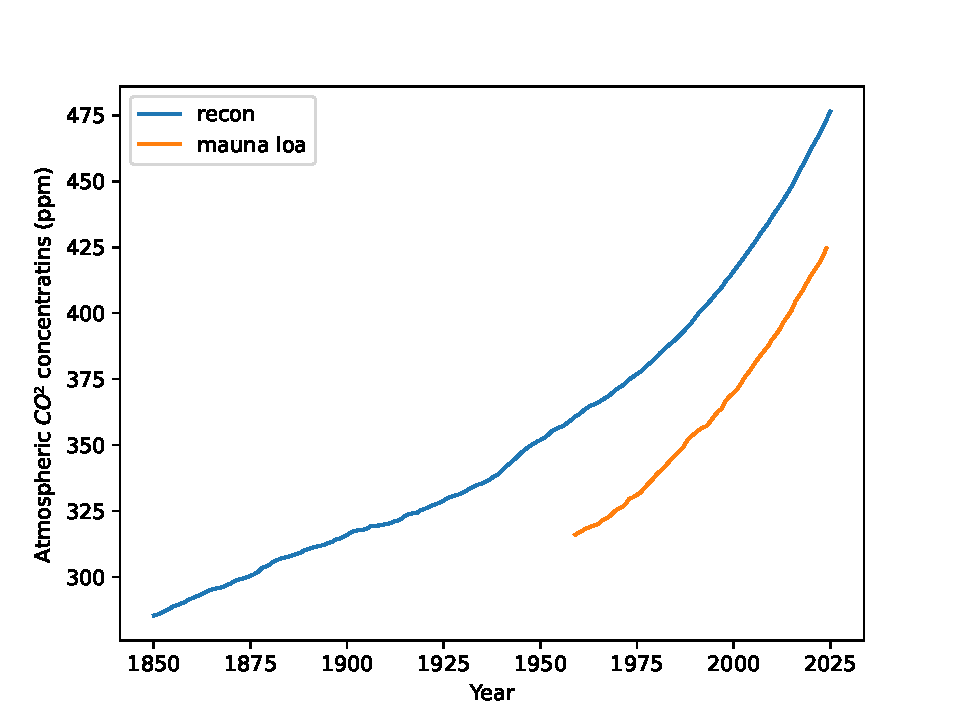
\includegraphics[scale=0.5]{../img/recon3.pdf}
  \caption{Reconstruction from 1850, starting at 285 ppm.}
  \label{fig:shoot}
\end{figure}

If we try to create a physical model of what is happening we must of
course explain where our emissions go. We can not simply say that they
disappear; since we obviously emit them in the atmosphere we need to
explain why they do not contribute much to the increase that we have
seen. If we build such a model we should not be surprised if the
temperature plays a significant role and even explains a large part of
the increase of carbon dioxide in the atmosphere.

\section*{Summary}

I argue that if should understand the reason behind the increase in
carbon dioxide levels in the atmosphere, we need to take temperature
into account. The view that it only contribute to the variability in
yearly changes but not in the long term increase is to simplify
matters. In the end, I think the temperature increase that we have
seen during the last hundred years can explain a large part of the
atmospheric in crease that is observed, what is your guess: 10, 20 or
50 percent?

If it turns out that emissions play a minor role in the increasing
carbon dioxide levels in the atmosphere we might have to reconsider
much of today's climate policies.


\end{document}
